% Options for packages loaded elsewhere
\PassOptionsToPackage{unicode}{hyperref}
\PassOptionsToPackage{hyphens}{url}
%
\documentclass[
]{article}
\usepackage{lmodern}
\usepackage{amsmath}
\usepackage{ifxetex,ifluatex}
\ifnum 0\ifxetex 1\fi\ifluatex 1\fi=0 % if pdftex
  \usepackage[T1]{fontenc}
  \usepackage[utf8]{inputenc}
  \usepackage{textcomp} % provide euro and other symbols
  \usepackage{amssymb}
\else % if luatex or xetex
  \usepackage{unicode-math}
  \defaultfontfeatures{Scale=MatchLowercase}
  \defaultfontfeatures[\rmfamily]{Ligatures=TeX,Scale=1}
\fi
% Use upquote if available, for straight quotes in verbatim environments
\IfFileExists{upquote.sty}{\usepackage{upquote}}{}
\IfFileExists{microtype.sty}{% use microtype if available
  \usepackage[]{microtype}
  \UseMicrotypeSet[protrusion]{basicmath} % disable protrusion for tt fonts
}{}
\makeatletter
\@ifundefined{KOMAClassName}{% if non-KOMA class
  \IfFileExists{parskip.sty}{%
    \usepackage{parskip}
  }{% else
    \setlength{\parindent}{0pt}
    \setlength{\parskip}{6pt plus 2pt minus 1pt}}
}{% if KOMA class
  \KOMAoptions{parskip=half}}
\makeatother
\usepackage{xcolor}
\IfFileExists{xurl.sty}{\usepackage{xurl}}{} % add URL line breaks if available
\IfFileExists{bookmark.sty}{\usepackage{bookmark}}{\usepackage{hyperref}}
\hypersetup{
  pdftitle={Exercise 3},
  pdfauthor={Yuting Huang, Jipeng Cheng, Weidi Hou},
  hidelinks,
  pdfcreator={LaTeX via pandoc}}
\urlstyle{same} % disable monospaced font for URLs
\usepackage[margin=1in]{geometry}
\usepackage{graphicx}
\makeatletter
\def\maxwidth{\ifdim\Gin@nat@width>\linewidth\linewidth\else\Gin@nat@width\fi}
\def\maxheight{\ifdim\Gin@nat@height>\textheight\textheight\else\Gin@nat@height\fi}
\makeatother
% Scale images if necessary, so that they will not overflow the page
% margins by default, and it is still possible to overwrite the defaults
% using explicit options in \includegraphics[width, height, ...]{}
\setkeys{Gin}{width=\maxwidth,height=\maxheight,keepaspectratio}
% Set default figure placement to htbp
\makeatletter
\def\fps@figure{htbp}
\makeatother
\setlength{\emergencystretch}{3em} % prevent overfull lines
\providecommand{\tightlist}{%
  \setlength{\itemsep}{0pt}\setlength{\parskip}{0pt}}
\setcounter{secnumdepth}{-\maxdimen} % remove section numbering
\usepackage{booktabs}
\usepackage{longtable}
\usepackage{array}
\usepackage{multirow}
\usepackage{wrapfig}
\usepackage{float}
\usepackage{colortbl}
\usepackage{pdflscape}
\usepackage{tabu}
\usepackage{threeparttable}
\usepackage{threeparttablex}
\usepackage[normalem]{ulem}
\usepackage{makecell}
\usepackage{xcolor}
\ifluatex
  \usepackage{selnolig}  % disable illegal ligatures
\fi

\title{Exercise 3}
\author{Yuting Huang, Jipeng Cheng, Weidi Hou}
\date{4/5/2022}

\begin{document}
\maketitle

\hypertarget{problem-1-what-causes-what}{%
\subsubsection{Problem 1: What causes
what?}\label{problem-1-what-causes-what}}

\textbf{Question 1. Why can't I just get data from a few different
cities and run the regression of ``Crime'' on ``Police'' to understand
how more cops in the streets affect crime? (``Crime'' refers to some
measure of crime rate and ``Police'' measures the number of cops in a
city.)}

answer: In this question of ``Crime'' and ``Police'', there is a problem
of endogeneity circle. if we use the simple linear regresstion model
\[y=beta_1+beta_2 * x+u\], there is a problem of endogeneity, i.e.
E(xu)≠0. Under is circumstance, inconsistency of OLS arises due to the
fact that changes in x(police force) are associated not only with chages
in y(crime), but also change in u.

\textbf{Question2. How were the researchers from UPenn able to isolate
this effect? Briefly describe their approach and discuss their result in
the ``Table 2'' below, from the researchers' paper.}

answer: In the paper, the authors use a ``high-alert periods'' dummy
variable to break the circle of endogeneity to estimate the effect of
police on crime. The reason why the authors choose ``high-alert
periods'' is that the primary purpose of the HSAS is to inform and
coordinate the antiterrorism efforts of all federal agencies. So, it the
level of alert will directly impact the number of police on the specific
district. In addition, the authors use daily data to make sure the
``treatment windows'' are short. Plus, the choosing data includes the
information repeated terror alert, so it reduces the possibility of
spurious correlation. Furthermore, the model also uses a ``Metro
ridership'' variable to test whether there is a correlation between
tourism and crime. At last, the authors use dummy variables for each day
of the week to control for day effects.

From the Table 2 column 1, the coefficient on the alert level is
statistically significant at the 5 percent level and indicates that on
high-alert days, total crimes decrease by an average of seven crimes per
day, or approximately 6.6 percent. From the Table 2 column 2, we verify
that high-alert levels are not being confounded with tourism levels by
including logged midday Metro ridership directly in the regression. The
coefficient on the alert level is slightly smaller, at -6.2 crimes per
day. We also find that increased Metro ridership is correlated with an
increase in crime. The increase, however, is very small, a 10 percent
increase in Metro ridership increases the number of crimes by only 1.7
per day on average. Thus, given that midday Metro ridership is a good
proxy for tourism, changes in the number of tourists cannot explain the
systematic change in crime that we estimate.

\textbf{Question3. Why did they have to control for Metro ridership?
What was that trying to capture?}

In order to test a hypothesis that tourism is reduced on high-alert
days, and as a result, there are fewer potential victims, which leads to
fewer crimes.

\textbf{Question4. Below I am showing you ``Table 4'' from the
researchers' paper. Just focus on the first column of the table. Can you
describe the model being estimated here? What is the conclusion?}

The model in table 4 includes district fixed effects in order to
distinguish the peculiar crime pattern of each district, and all
regressions contain day-of-the-week fixed effects. The dependent
variable is daily crime totals by district. From Table 4, During periods
of high alert, crime in the National Mall area decreases by 2.62 crimes
per day. Crime also decreases in the other districts, by 0.571 crimes
per day, but this effect is not statistically significant. Since there
are 17.1 crimes on the district 1, the declination during high-alert
days is approximately 15 percent, which means almost one-half of the
total crime decline during high-alert periods is concentrated in
District 1. In addition, The result elasticity of crime with respect to
police is -0.3, which is consistent with other researchers' results.

\hypertarget{problem-2-tree-modeling-dengue-cases}{%
\subsubsection{Problem 2: Tree modeling: dengue
cases}\label{problem-2-tree-modeling-dengue-cases}}

\begin{table}

\caption{\label{tab:unnamed-chunk-1}The RMSEs of Models}
\centering
\begin{tabular}[t]{r|r|r}
\hline
dengue\_tree & dengue\_forest & dengue\_boost\\
\hline
45.17933 & 45.72094 & 44.82081\\
\hline
\end{tabular}
\end{table}

The results suggest that random forests mode have the best performance
on the testing data.

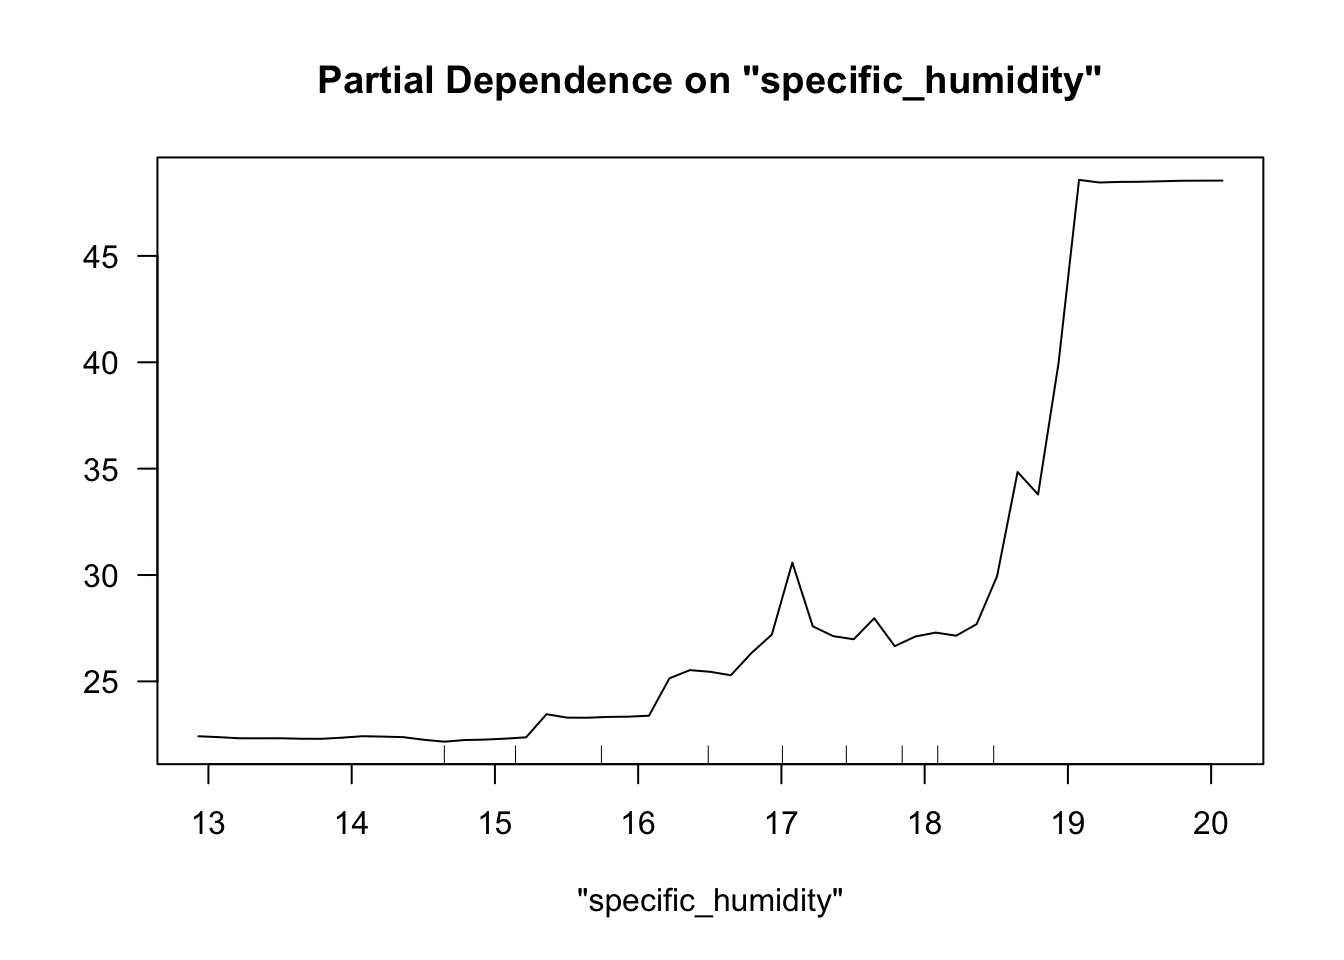
\includegraphics{Exercise_3_files/figure-latex/unnamed-chunk-2-1.pdf}
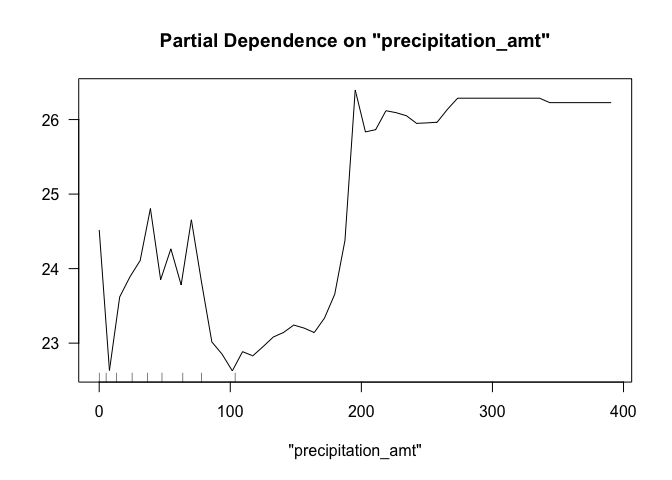
\includegraphics{Exercise_3_files/figure-latex/unnamed-chunk-2-2.pdf}
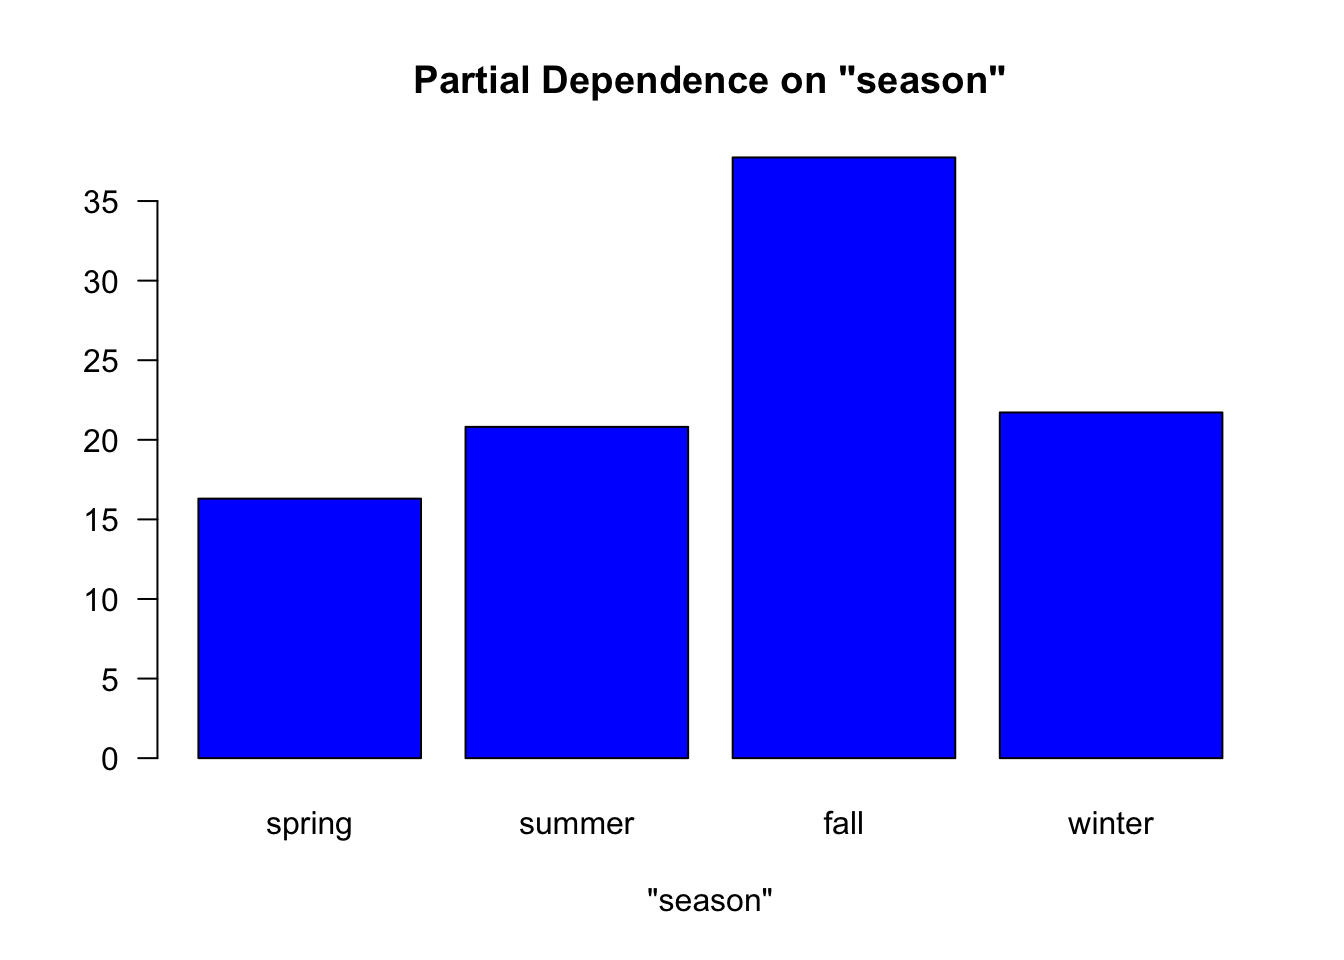
\includegraphics{Exercise_3_files/figure-latex/unnamed-chunk-2-3.pdf}

\hypertarget{problem-3-predictive-model-building-green-certification}{%
\subsubsection{Problem 3: Predictive model building: green
certification}\label{problem-3-predictive-model-building-green-certification}}

\hypertarget{overview}{%
\paragraph{Overview}\label{overview}}

As landlords and renters, what they mostly care about is their possible
revenue per square foot per calendar year. As we all know, their revenue
depends on many factors, such as the age, facilities, amenities ,
leasing rate and so on. Nowadays, people pay more attention on their
living environment when renting a house, such as whether this landload
has a green certification. Therefore, it's meaningful to do some
research on the relationship between rental income and green
certification.

In our report, we build our best predictive model possible for revenue
per square foot per calendar year and to use this model to quantify the
average change in rental income per square foot associated with green
certification, holding other features of the building constant.

\hypertarget{data-and-research-design}{%
\paragraph{Data and research design}\label{data-and-research-design}}

\hypertarget{data}{%
\subparagraph{Data}\label{data}}

In our raw data set, there are 7,894 data points. We first filter out
those missing data. Now, our new greenbuildings data set has 7820 data
points.

\hypertarget{predictive-variable-and-features}{%
\subparagraph{Predictive variable and
features}\label{predictive-variable-and-features}}

The predictive variable is revenue per square foot per year, which is
the product of two terms: rent and leasing\_rate.

The features used to build our model are:

\begin{verbatim}
(1) CS.PropertyID: the building's unique identifier in the database.

(2) cluster: an identifier for the building cluster, with each cluster containing one green-certified building and at least one other non-green-certified building within a quarter-mile radius of the cluster center.

(3) size: the total square footage of available rental space in the building.

(4) empl.gr: the year-on-year growth rate in employment in the building's geographic region.

(5) Rent: the rent charged to tenants in the building, in dollars per square foot per calendar year.

(6) leasing.rate: a measure of occupancy; the fraction of the building's available space currently under lease.

(7) stories: the height of the building in stories.

(8) age: the age of the building in years.

(9) renovated: whether the building has undergone substantial renovations during its lifetime.

(10) (11) class.a, class.b: indicators for two classes of building quality (the third is Class C). These are relative classifications within a specific market. Class A buildings are generally the highest-quality properties in a given market. Class B buildings are a notch down, but still of reasonable quality. Class C buildings are the least desirable properties in a given market.

(12) green.rating: an indicator for whether the building is either LEED- or EnergyStar-certified.

(13) LEED, Energystar: indicators for the two specific kinds of green certifications.

(14) net: an indicator as to whether the rent is quoted on a "net contract" basis. Tenants with net-rental contracts pay their own utility costs, which are otherwise included in the quoted rental price.

(15) amenities: an indicator of whether at least one of the following amenities is available on-site: bank, convenience store, dry cleaner, restaurant, retail shops, fitness center.

(16) cd.total.07: number of cooling degree days in the building's region in 2007. A degree day is a measure of demand for energy; higher values mean greater demand. Cooling degree days are measured relative to a baseline outdoor temperature, below which a building needs no cooling.

(17) hd.total07: number of heating degree days in the building's region in 2007. Heating degree days are also measured relative to a baseline outdoor temperature, above which a building needs no heating.

(18) total.dd.07: the total number of degree days (either heating or cooling) in the building's region in 2007.

(19) Precipitation: annual precipitation in inches in the building's geographic region.

(20) Gas.Costs: a measure of how much natural gas costs in the building's geographic region.

(21)Electricity.Costs: a measure of how much electricity costs in the building's geographic region.

(22)City_Market_Rent: a measure of average rent per square-foot per calendar year in the building's local market.
\end{verbatim}

\hypertarget{research-design}{%
\paragraph{Research design}\label{research-design}}

\begin{verbatim}
## [1] 7.473907
\end{verbatim}

\begin{verbatim}
## Distribution not specified, assuming gaussian ...
\end{verbatim}

\begin{verbatim}
## [1] 9.053765
\end{verbatim}

By using the tree model to build our predictive model, we identify the
association between rental revenue and green certification. We first
split the new greenbuilds data set into training and test test, then we
use two different tree methods: random forest and boosted regression
trees to build our model. Then we calculate the out of sample RMSE. The
result shows that the RMSE of the random forest model is lower that the
one using boosted regression trees. Therefore, we choose to use random
forest method.

\hypertarget{results}{%
\paragraph{Results}\label{results}}

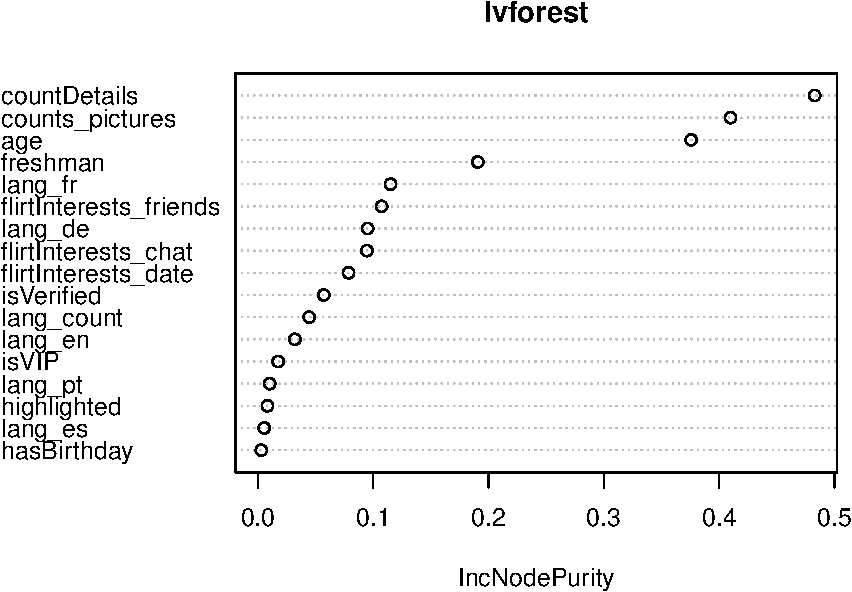
\includegraphics{Exercise_3_files/figure-latex/unnamed-chunk-6-1.pdf}
\textbf{Figure 1:} Figure of all features used in our predictive model
descending by importance.

From Figure 1, we found that the most important features that landlords
should consider are ``size, age, stories'', these variables seems to be
the most important. However, the ``green\_rating'' variable is not that
important from our observation.

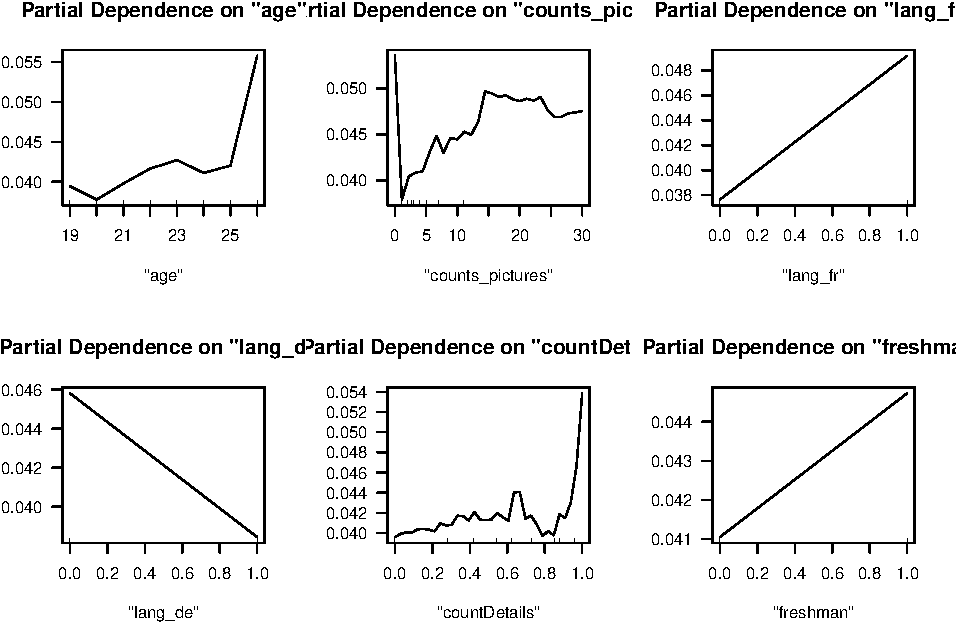
\includegraphics{Exercise_3_files/figure-latex/unnamed-chunk-7-1.pdf}

\textbf{Figure 2:} Impact of Green Certifications on Revenue

From the box plot including the information between revenue and
green\_rating, the average rent per square foot is around 20 for
buildings with a green certification, and around 24 for those without a
certification. Therefore, we didn't find significant difference between
buildings with or without green certification.

\begin{verbatim}
## # A tibble: 2 x 2
##   green_rating `mean(predict_rent)`
##          <int>                <dbl>
## 1            0                 24.3
## 2            1                 27.1
\end{verbatim}

\textbf{Table 1:} The average change in revenue per square foot related
to green certification

We then calculate the average change in revenue per square foot for
buildings with or without green certification. From the table above, we
found that buildings with green certification get more revenue than
those without green certification, but the impact is small, considering
the difference is 2 unit.

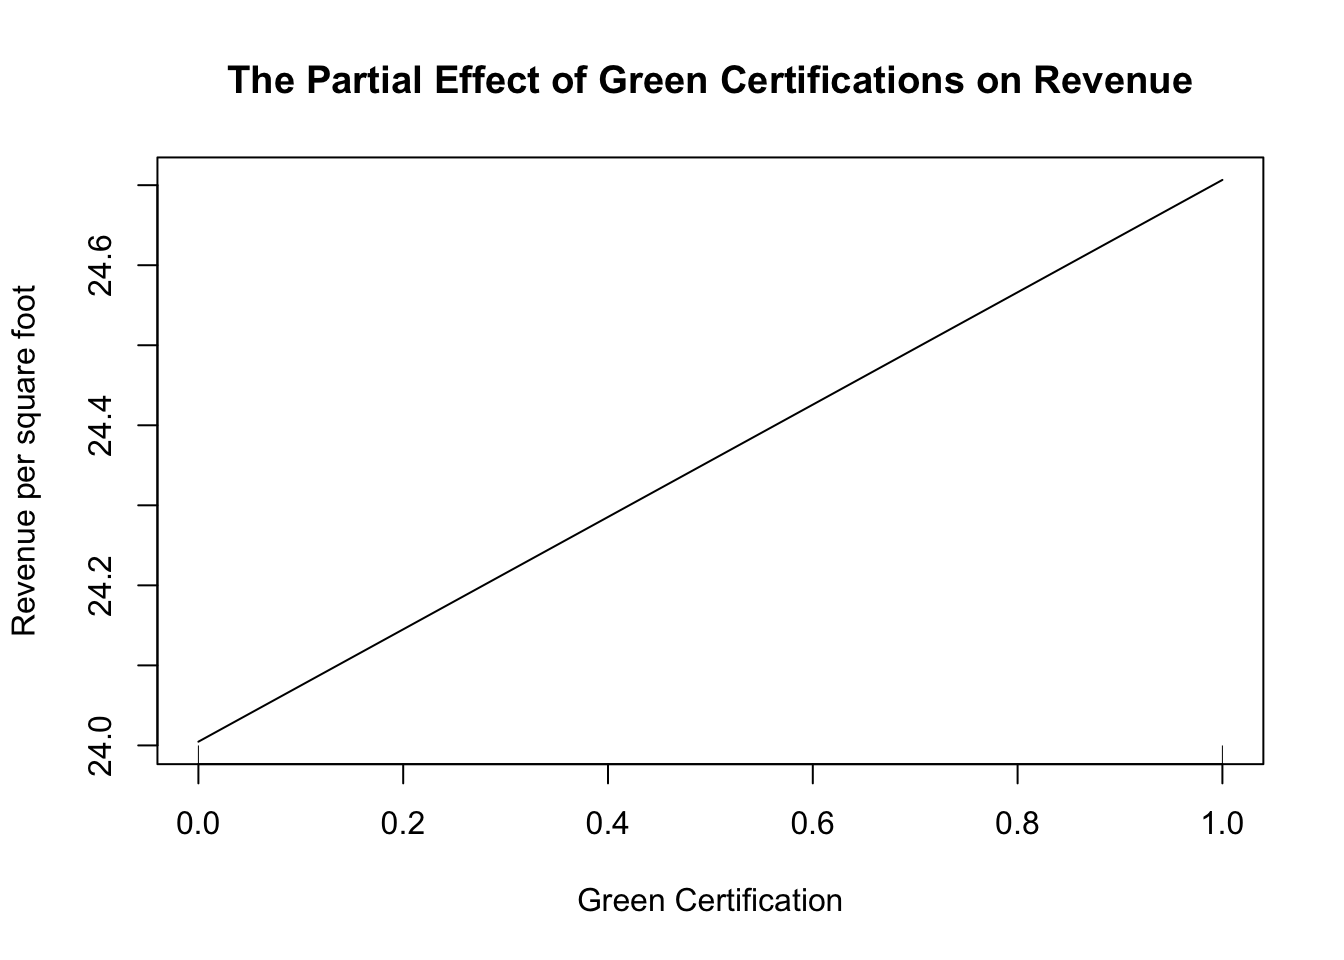
\includegraphics{Exercise_3_files/figure-latex/unnamed-chunk-9-1.pdf}

\textbf{Figure 3:} Partial Effect of Green Certifications on Revenue

From the partial effect figure of green certification on revenue per
square foot, we found a positive association between revenue and green
certification, which means green certification has some good impact on
revenue.

\hypertarget{conclusion}{%
\paragraph{Conclusion}\label{conclusion}}

From our analysis, we build the model using random forest to estimate
the association between green certification and revenue per square foot.
From our results, we found that green certification has some positive
impact on revenue, but the impact isn't very significant. In addition,
we found that these variables ``size, age, stories'' have more impact on
revenue. Based on our research, the landlords should weigh the pros and
cons of getting a green certification, thinking critically about the
cost and revenue change of getting a green certification. If they figure
that the income change isn't overweigh the cost of getting a
certification, they should focus on other features, which have more
important impact on revenue.

\hypertarget{problem-4-predictive-model-building-california-housing}{%
\subsubsection{Problem 4: Predictive model building: California
housing}\label{problem-4-predictive-model-building-california-housing}}

Our purpose is to build the best predictive model to forecast the median
house value in California. According to the topic description, in the
beginning, we have to conduct standardized processing for ``totalRooms''
and totalBedrooms" by creating the new variables including ``sdrooms''
and ``sdbedrooms''. Then we utilized three different methods including
Step wise, Random Forecast and boost, to build the best predictive
model.

Now, we estimate their RMSE to find out which model is our best
predictive model.

\begin{table}

\caption{\label{tab:unnamed-chunk-12}The RMSEs of Models}
\centering
\begin{tabular}[t]{r|r|r|r|r}
\hline
lm\_medium & lm\_step & dengue\_boost & cahousing\_forest & cahousing\_boost\\
\hline
72581.48 & 72431.48 & 62329.03 & 50900.29 & 72813.14\\
\hline
\end{tabular}
\end{table}

According to our results, we can find the Random Forecast model has
lower RMSE, so we use this to build our best predictive model.

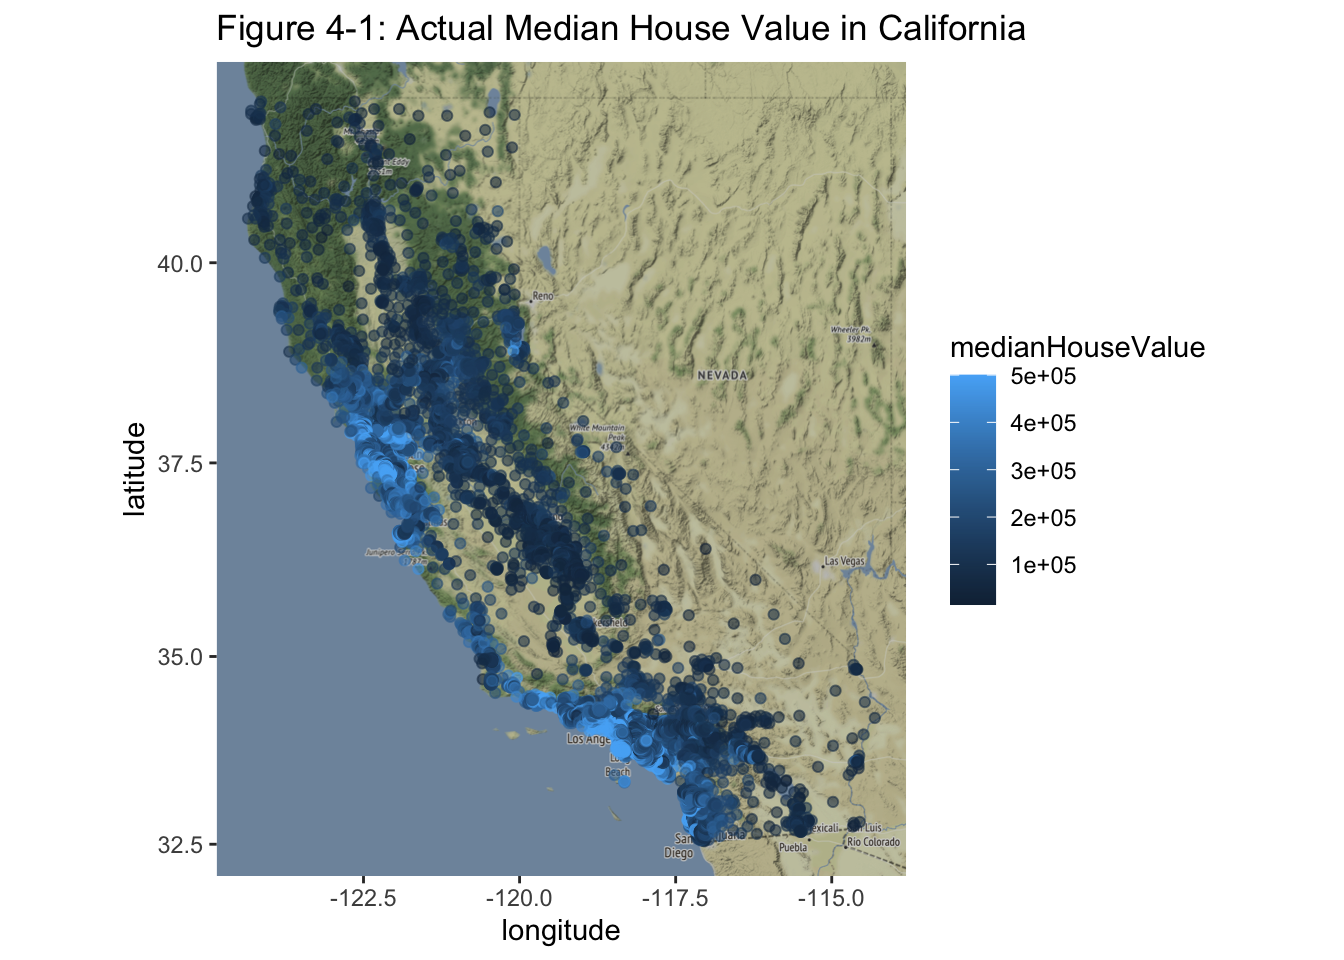
\includegraphics{Exercise_3_files/figure-latex/unnamed-chunk-13-1.pdf}
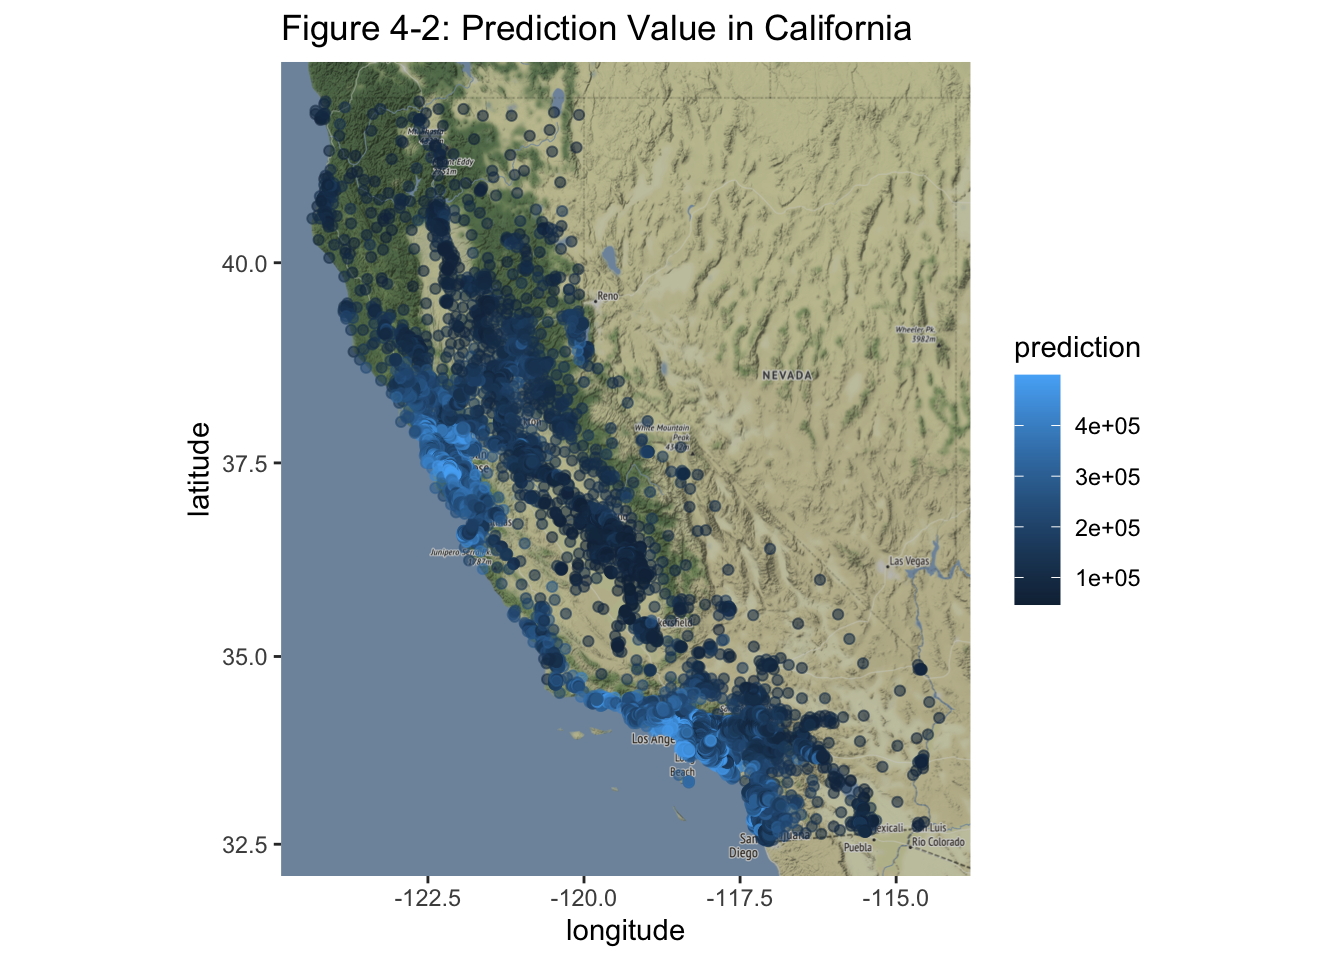
\includegraphics{Exercise_3_files/figure-latex/unnamed-chunk-13-2.pdf}
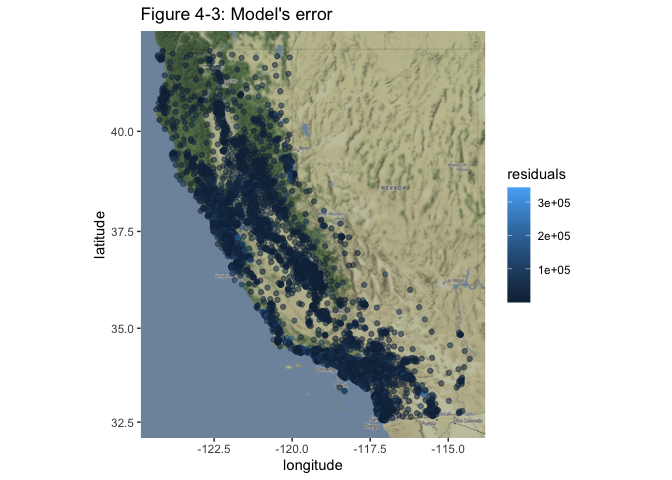
\includegraphics{Exercise_3_files/figure-latex/unnamed-chunk-13-3.pdf}

We can find that above graphs are perform well, because Figure1: Actual
Median House Value in California are almost match with Figure 4-2:
Prediction Value in California. Therefore, we can indicate the random
forest is the best predictive model in this case. In conclusion, our
predictive model is effective, then we may use this predictive model to
forecast other states or area in United State.

\end{document}
